%%
% SigLog paper on HoTT
% May 2014
% IHP
%%
\documentclass[11pt]{article}
\usepackage{amsmath}
\usepackage{amssymb,latexsym}
\usepackage{amsthm}
\usepackage{bm}
\message{<Paul Taylor's Proof Trees, 2 August 1996>}
%% Build proof tree for Natural Deduction, Sequent Calculus, etc.
%% WITH SHORTENING OF PROOF RULES!
%% Paul Taylor, begun 10 Oct 1989
%% *** THIS IS ONLY A PRELIMINARY VERSION AND THINGS MAY CHANGE! ***
%%
%% 2 Aug 1996: fixed \mscount and \proofdotnumber
%%
%%      \prooftree
%%              hyp1            produces:
%%              hyp2
%%              hyp3            hyp1    hyp2    hyp3
%%      \justifies              -------------------- rulename
%%              concl                   concl
%%      \thickness=0.08em
%%      \shiftright 2em
%%      \using
%%              rulename
%%      \endprooftree
%%
%% where the hypotheses may be similar structures or just formulae.
%%
%% To get a vertical string of dots instead of the proof rule, do
%%
%%      \prooftree                      which produces:
%%              [hyp]
%%      \using                                  [hyp]
%%              name                              .
%%      \proofdotseparation=1.2ex                 .name
%%      \proofdotnumber=4                         .
%%      \leadsto                                  .
%%              concl                           concl
%%      \endprooftree
%%
%% Within a prooftree, \[ and \] may be used instead of \prooftree and
%% \endprooftree; this is not permitted at the outer level because it
%% conflicts with LaTeX. Also,
%%      \Justifies
%% produces a double line. In LaTeX you can use \begin{prooftree} and
%% \end{prootree} at the outer level (however this will not work for the inner
%% levels, but in any case why would you want to be so verbose?).
%%
%% All of of the keywords except \prooftree and \endprooftree are optional
%% and may appear in any order. They may also be combined in \newcommand's
%% eg "\def\Cut{\using\sf cut\thickness.08em\justifies}" with the abbreviation
%% "\prooftree hyp1 hyp2 \Cut \concl \endprooftree". This is recommended and
%% some standard abbreviations will be found at the end of this file.
%%
%% \thickness specifies the breadth of the rule in any units, although
%% font-relative units such as "ex" or "em" are preferable.
%% It may optionally be followed by "=".
%% \proofrulebreadth=.08em or \setlength\proofrulebreadth{.08em} may also be
%% used either in place of \thickness or globally; the default is 0.04em.
%% \proofdotseparation and \proofdotnumber control the size of the
%% string of dots
%%
%% If proof trees and formulae are mixed, some explicit spacing is needed,
%% but don't put anything to the left of the left-most (or the right of
%% the right-most) hypothesis, or put it in braces, because this will cause
%% the indentation to be lost.
%%
%% By default the conclusion is centered wrt the left-most and right-most
%% immediate hypotheses (not their proofs); \shiftright or \shiftleft moves
%% it relative to this position. (Not sure about this specification or how
%% it should affect spreading of proof tree.)
%
% global assignments to dimensions seem to have the effect of stretching
% diagrams horizontally.
%
%%==========================================================================

\def\introrule{{\cal I}}\def\elimrule{{\cal E}}%%
\def\andintro{\using{\land}\introrule\justifies}%%
\def\impelim{\using{\Rightarrow}\elimrule\justifies}%%
\def\allintro{\using{\forall}\introrule\justifies}%%
\def\allelim{\using{\forall}\elimrule\justifies}%%
\def\falseelim{\using{\bot}\elimrule\justifies}%%
\def\existsintro{\using{\exists}\introrule\justifies}%%

%% #1 is meant to be 1 or 2 for the first or second formula
\def\andelim#1{\using{\land}#1\elimrule\justifies}%%
\def\orintro#1{\using{\lor}#1\introrule\justifies}%%

%% #1 is meant to be a label corresponding to the discharged hypothesis/es
\def\impintro#1{\using{\Rightarrow}\introrule_{#1}\justifies}%%
\def\orelim#1{\using{\lor}\elimrule_{#1}\justifies}%%
\def\existselim#1{\using{\exists}\elimrule_{#1}\justifies}

%%==========================================================================

\newdimen\proofrulebreadth \proofrulebreadth=.05em
\newdimen\proofdotseparation \proofdotseparation=1.25ex
\newdimen\proofrulebaseline \proofrulebaseline=2ex
\newcount\proofdotnumber \proofdotnumber=3
\let\then\relax
\def\hfi{\hskip0pt plus.0001fil}
\mathchardef\squigto="3A3B
%
% flag where we are
\newif\ifinsideprooftree\insideprooftreefalse
\newif\ifonleftofproofrule\onleftofproofrulefalse
\newif\ifproofdots\proofdotsfalse
\newif\ifdoubleproof\doubleprooffalse
\let\wereinproofbit\relax
%
% dimensions and boxes of bits
\newdimen\shortenproofleft
\newdimen\shortenproofright
\newdimen\proofbelowshift
\newbox\proofabove
\newbox\proofbelow
\newbox\proofrulename
%
% miscellaneous commands for setting values
\def\shiftproofbelow{\let\next\relax\afterassignment\setshiftproofbelow\dimen0 }
\def\shiftproofbelowneg{\def\next{\multiply\dimen0 by-1 }%
\afterassignment\setshiftproofbelow\dimen0 }
\def\setshiftproofbelow{\next\proofbelowshift=\dimen0 }
\def\setproofrulebreadth{\proofrulebreadth}

%=============================================================================
\def\prooftree{% NESTED ZERO (\ifonleftofproofrule)
%
% first find out whether we're at the left-hand end of a proof rule
\ifnum  \lastpenalty=1
\then   \unpenalty
\else   \onleftofproofrulefalse
\fi
%
% some space on left (except if we're on left, and no infinity for outermost)
\ifonleftofproofrule
\else   \ifinsideprooftree
        \then   \hskip.5em plus1fil
        \fi
\fi
%
% begin our proof tree environment
\bgroup% NESTED ONE (\proofbelow, \proofrulename, \proofabove,
%               \shortenproofleft, \shortenproofright, \proofrulebreadth)
\setbox\proofbelow=\hbox{}\setbox\proofrulename=\hbox{}%
\let\justifies\proofover\let\leadsto\proofoverdots\let\Justifies\proofoverdbl
\let\using\proofusing\let\[\prooftree
\ifinsideprooftree\let\]\endprooftree\fi
\proofdotsfalse\doubleprooffalse
\let\thickness\setproofrulebreadth
\let\shiftright\shiftproofbelow \let\shift\shiftproofbelow
\let\shiftleft\shiftproofbelowneg
\let\ifwasinsideprooftree\ifinsideprooftree
\insideprooftreetrue
%
% now begin to set the top of the rule (definitions local to it)
\setbox\proofabove=\hbox\bgroup$\displaystyle % NESTED TWO
\let\wereinproofbit\prooftree
%
% these local variables will be copied out:
\shortenproofleft=0pt \shortenproofright=0pt \proofbelowshift=0pt
%
% flags to enable inner proof tree to detect if on left:
\onleftofproofruletrue\penalty1
}

%=============================================================================
% end whatever box and copy crucial values out of it
\def\eproofbit{% NESTED TWO
%
% various hacks applicable to hypothesis list 
\ifx    \wereinproofbit\prooftree
\then   \ifcase \lastpenalty
        \then   \shortenproofright=0pt  % 0: some other object, no indentation
        \or     \unpenalty\hfil         % 1: empty hypotheses, just glue
        \or     \unpenalty\unskip       % 2: just had a tree, remove glue
        \else   \shortenproofright=0pt  % eh?
        \fi
\fi
%
% pass out crucial values from scope
\global\dimen0=\shortenproofleft
\global\dimen1=\shortenproofright
\global\dimen2=\proofrulebreadth
\global\dimen3=\proofbelowshift
\global\dimen4=\proofdotseparation
\global\count255=\proofdotnumber
%
% end the box
$\egroup  % NESTED ONE
%
% restore the values
\shortenproofleft=\dimen0
\shortenproofright=\dimen1
\proofrulebreadth=\dimen2
\proofbelowshift=\dimen3
\proofdotseparation=\dimen4
\proofdotnumber=\count255
}

%=============================================================================
\def\proofover{% NESTED TWO
\eproofbit % NESTED ONE
\setbox\proofbelow=\hbox\bgroup % NESTED TWO
\let\wereinproofbit\proofover
$\displaystyle
}%
%
%=============================================================================
\def\proofoverdbl{% NESTED TWO
\eproofbit % NESTED ONE
\doubleprooftrue
\setbox\proofbelow=\hbox\bgroup % NESTED TWO
\let\wereinproofbit\proofoverdbl
$\displaystyle
}%
%
%=============================================================================
\def\proofoverdots{% NESTED TWO
\eproofbit % NESTED ONE
\proofdotstrue
\setbox\proofbelow=\hbox\bgroup % NESTED TWO
\let\wereinproofbit\proofoverdots
$\displaystyle
}%
%
%=============================================================================
\def\proofusing{% NESTED TWO
\eproofbit % NESTED ONE
\setbox\proofrulename=\hbox\bgroup % NESTED TWO
\let\wereinproofbit\proofusing
\kern0.3em$
}

%=============================================================================
\def\endprooftree{% NESTED TWO
\eproofbit % NESTED ONE
% \dimen0 =     length of proof rule
% \dimen1 =     indentation of conclusion wrt rule
% \dimen2 =     new \shortenproofleft, ie indentation of conclusion
% \dimen3 =     new \shortenproofright, ie
%                space on right of conclusion to end of tree
% \dimen4 =     space on right of conclusion below rule
  \dimen5 =0pt% spread of hypotheses
% \dimen6, \dimen7 = height & depth of rule
%
% length of rule needed by proof above
\dimen0=\wd\proofabove \advance\dimen0-\shortenproofleft
\advance\dimen0-\shortenproofright
%
% amount of spare space below
\dimen1=.5\dimen0 \advance\dimen1-.5\wd\proofbelow
\dimen4=\dimen1
\advance\dimen1\proofbelowshift \advance\dimen4-\proofbelowshift
%
% conclusion sticks out to left of immediate hypotheses
\ifdim  \dimen1<0pt
\then   \advance\shortenproofleft\dimen1
        \advance\dimen0-\dimen1
        \dimen1=0pt
%       now it sticks out to left of tree!
        \ifdim  \shortenproofleft<0pt
        \then   \setbox\proofabove=\hbox{%
                        \kern-\shortenproofleft\unhbox\proofabove}%
                \shortenproofleft=0pt
        \fi
\fi
%
% and to the right
\ifdim  \dimen4<0pt
\then   \advance\shortenproofright\dimen4
        \advance\dimen0-\dimen4
        \dimen4=0pt
\fi
%
% make sure enough space for label
\ifdim  \shortenproofright<\wd\proofrulename
\then   \shortenproofright=\wd\proofrulename
\fi
%
% calculate new indentations
\dimen2=\shortenproofleft \advance\dimen2 by\dimen1
\dimen3=\shortenproofright\advance\dimen3 by\dimen4
%
% make the rule or dots, with name attached
\ifproofdots
\then
        \dimen6=\shortenproofleft \advance\dimen6 .5\dimen0
        \setbox1=\vbox to\proofdotseparation{\vss\hbox{$\cdot$}\vss}%
        \setbox0=\hbox{%
                \advance\dimen6-.5\wd1
                \kern\dimen6
                $\vcenter to\proofdotnumber\proofdotseparation
                        {\leaders\box1\vfill}$%
                \unhbox\proofrulename}%
\else   \dimen6=\fontdimen22\the\textfont2 % height of maths axis
        \dimen7=\dimen6
        \advance\dimen6by.5\proofrulebreadth
        \advance\dimen7by-.5\proofrulebreadth
        \setbox0=\hbox{%
                \kern\shortenproofleft
                \ifdoubleproof
                \then   \hbox to\dimen0{%
                        $\mathsurround0pt\mathord=\mkern-6mu%
                        \cleaders\hbox{$\mkern-2mu=\mkern-2mu$}\hfill
                        \mkern-6mu\mathord=$}%
                \else   \vrule height\dimen6 depth-\dimen7 width\dimen0
                \fi
                \unhbox\proofrulename}%
        \ht0=\dimen6 \dp0=-\dimen7
\fi
%
% set up to centre outermost tree only
\let\doll\relax
\ifwasinsideprooftree
\then   \let\VBOX\vbox
\else   \ifmmode\else$\let\doll=$\fi
        \let\VBOX\vcenter
\fi
% this \vbox or \vcenter is the actual output:
\VBOX   {\baselineskip\proofrulebaseline \lineskip.2ex
        \expandafter\lineskiplimit\ifproofdots0ex\else-0.6ex\fi
        \hbox   spread\dimen5   {\hfi\unhbox\proofabove\hfi}%
        \hbox{\box0}%
        \hbox   {\kern\dimen2 \box\proofbelow}}\doll%
%
% pass new indentations out of scope
\global\dimen2=\dimen2
\global\dimen3=\dimen3
\egroup % NESTED ZERO
\ifonleftofproofrule
\then   \shortenproofleft=\dimen2
\fi
\shortenproofright=\dimen3
%
% some space on right and flag we've just made a tree
\onleftofproofrulefalse
\ifinsideprooftree
\then   \hskip.5em plus 1fil \penalty2
\fi
}

%==========================================================================
% IDEAS
% 1.    Specification of \shiftright and how to spread trees.
% 2.    Spacing command \m which causes 1em+1fil spacing, over-riding
%       exisiting space on sides of trees and not affecting the
%       detection of being on the left or right.
% 3.    Hack using \@currenvir to detect LaTeX environment; have to
%       use \aftergroup to pass \shortenproofleft/right out.
% 4.    (Pie in the sky) detect how much trees can be "tucked in"
% 5.    Discharged hypotheses (diagonal lines).

\usepackage[all,cmtip]{xy}
\input{diagxy}
\CompileMatrices       
\usepackage{url}
\usepackage{tikz}
\usepackage{pdfpages}

\usepackage[color=green!40]{todonotes}



% categories
\newcommand{\C}{\ensuremath{\mathbb{C}}}
\newcommand{\B}{\ensuremath{\mathbb{B}}}
\newcommand{\N}{\ensuremath{\mathbb{N}}}
\newcommand{\T}{\ensuremath{\mathbb{T}}}
\newcommand{\CC}{\ensuremath{\mathcal{C}}}
\newcommand{\BB}{\ensuremath{\mathcal{B}}}
%\newcommand{\EE}{\ensuremath{\mathcal{E}}}
\newcommand{\psh}[1]{\ensuremath{\mathsf{Set}^{#1^{\mathrm{op}}}}}
\newcommand{\Set}{\ensuremath{\mathsf{Set}}}
\newcommand{\Cat}{\ensuremath{\mathsf{Cat}}}
\newcommand{\covpsh}[1]{\ensuremath{\mathsf{Set}^{#1}}}
%\renewcommand{\to}{\ensuremath{\rightarrow}}
\newcommand{\pocorner}[1][dr]{\save*!/#1+1.2pc/#1:(1,-1)@^{|-}\restore}
\newcommand{\pbcorner}[1][dr]{\save*!/#1-1.2pc/#1:(-1,1)@^{|-}\restore}
\newcommand{\y}{\ensuremath{\mathsf{y}}} % Yoneda embedding

% arrows
\newcommand{\hook}{\ensuremath{\hookrightarrow}}
\newcommand{\mono}{\ensuremath{\rightarrowtail}}
%\newcommand{\epi}{\ensuremath{\twoheadrightarrow}}


% cubical sets
\newcommand{\I}{\ensuremath{\mathrm{I}}}
\renewcommand{\H}{\ensuremath{\mathbb{H}}}
\newcommand{\HH}{\ensuremath{\mathcal{H}}}

% type theory
\newcommand{\G}{\ensuremath{\Gamma}}
\newcommand{\defeq}{=_{\mathrm{def}}}
\newcommand{\type}{\mathsf{type}}       
\newcommand{\types}[2]{#1 \vdash #2:\type}
\newcommand{\Gtypes}[1]{\types{\Gamma}{#1}}
\newcommand{\term}[2]{#1\,:\,#2}
\newcommand{\terms}[2]{#1 \vdash #2}
\newcommand{\Gterms}[1]{\terms{\Gamma}{#1}}
\newcommand{\ext}[2]{{#1\!\centerdot\! #2}}
\newcommand{\ty}{\ensuremath{\,:\,}}
\newcommand{\pair}[1]{\ensuremath{\langle #1\rangle}}
\newcommand{\exdot}{\ensuremath{\!\centerdot\!}}
\newcommand{\texdot}{\ensuremath{\centerdot}}

% Id types
\newcommand{\Id}{\mathsf{Id}}
\newcommand{\id}[1]{\Id_{#1}}
\newcommand{\refl}{\mathsf{refl}}
\newcommand{\rec}{\mathsf{rec}}
\newcommand{\idrec}{\mathsf{idrec}}
\newcommand{\jay}{\mathsf{j}}
\renewcommand{\i}{\mathsf{i}}

% Universe
\newcommand{\U}{\ensuremath{\mathcal{U}}}
\newcommand{\UU}{\ensuremath{\widetilde{\mathcal{U}}}}

% theorem styles
\newtheorem{theorem}{Theorem}
\newtheorem*{theorem*}{Theorem}
\newtheorem{proposition}[theorem]{Proposition} 
\newtheorem{lemma}[theorem]{Lemma}
\newtheorem{corollary}[theorem]{Corollary} 

\theoremstyle{remark}
\newtheorem{remark}[theorem]{Remark} 
\newtheorem*{remarks*}{Remarks}
\newtheorem{example}[theorem]{Example}

\theoremstyle{definition}
\newtheorem{definition}[theorem]{Definition}

%%%%%%%%%%%%%%%%%%%%%%%%%%%%%%%%%%%%%%%%%%%%%%%%%%%%
\begin{document}
%%%%%%%%%%%%%%%%%%%%%%%%%%%%%%%%%%%%%%%%%%%%%%%%%%%%

\title{Homotopy Type Theory and Univalent Foundations}
\author{Steve Awodey \and Robert Harper}
\date{\today}

\maketitle
%%%%%%%%%%%%%%%%%%%%%%%%%%%%%%%%%%%%%%%%%%%%%%%%%%%%

Homotopy Type Theory is an emerging unification of previously disparate frameworks for formalizing and mechanizing mathematics, one based on a computational conception of the type of a construction, the other based on a homotopical conception of the (homotopy) type of a space.  Indeed, the name ``homotopy type theory'' can be read in two ways, as ``(homotopy type) theory'' and ``homotopy (type theory)'', neatly summarizing the consolidation of ideas at the heart of the subject.  The computational notion of type has its origins in Brouwer's program of intuitionism, which sought to ground mathematics in the concept of an effective construction (one would say ``algorithm'' these days).  The homotopical notion of type emerges from abstract homotopy theory, in particular Grothendieck's conception of a space as an $\infty$-groupoid.  The former perspective was developed most fully by Per Martin-L\"{o}f, leading in particular to his Intuitionistic Theory of Types, on which the formal system of homotopy type theory is based.  The connection to homotopy theory was first hinted at in the groupoid interpretation of Hofmann and Streicher and then made explicit by Awodey and his students Lumsdaine and Warren, who showed that every type in Martin-L\"{o}f's system has the structure of an $\infty$-groupoid, and that the entire system can be interpreted in any Quillen model category, an abstract framework for doing homotopy theory.  The connection was clinched by Voevodsky's introduction of the \emph{univalence axiom}, which is motivated by the homotopical interpretation and relates the aforementioned identity type to the central notion of homotopy equivalence.

Because univalence plays such a central role, Voevodsky has suggested that the unification of the computational and homotopical perspectives be called the \emph{Univalent Unification} of two major lines of development in mathematics.  A critically important point is that the univalent unification is \emph{fully compatible} with classical mathematics; it does not involve any principles that are incompatible with classical reasoning, though it does, at the outset, avoid postulating axioms that are unnecessary for much of the development.  Indeed, the formal system of homotopy type theory contains within it the whole of ZF set theory, with or without the Axiom of Choice, and with or without the Law of the Excluded Middle, two principles that lie at the heart of classical mathematics and that have, regrettably, been obstacles to the kind of unification described here.  By not insisting on these axioms globally, it is possible to consider a far richer notion of type than has hitherto been possible in the computational setting, namely one in which types are abstract spaces that can have non-trivial higher-dimensional structure, as exemplified by familiar examples such as the $n$-spheres for all $n\geq 0$.  Rather than being ``coded up'' as certain structured sets representing certain conceptions of space, such as a topological space, these objects instead arise \emph{synthetically} within the theory.  They are characterized by their introductory and eliminatory forms (mapping-in and mapping-out properties, or universal properties), rather than by how they are constructed as sets.  This perspective greatly simplifies many familiar constructions in homotopy theory, such as homotopy groups, truncations, and Eilenberg-MacLane spaces, and supports remarkably simple and clear proofs of well-known results, such as calculations of the higher homotopy groups of the spheres.  In this way it is possible to unify standard, classical logic and set theory with constructive logic and type theory by regarding the former as the logic of a very special kind of objects (namely, sets), and the latter as the general logic that applies not only to sets (the $0$-level spaces), but also to the higher types of spaces.

What is it that makes the univalent unification possible?  Although it may be too early to formulate a single, deep
unifying principle, it is possible to make a few observations that will give the reader a sense of its inevitability.
First, all of the constructions of Intuitionistic Type Theory, including especially the previously enigmatic identity
type, are homotopy invariant, in the both sense that type families and mappings between types inherently respect
``paths'' in spaces, representing \emph{identifications} of points in the space, and that the formation of type-indexed
products and sums of types, which correspond to analogous constructions on spaces, respect the homotopically motivated
notion of type equivelence.  This invariance essentially follows from the basic fact that the important identity type,
taken as a whole, corresponds to the \emph{total path space} of a space (see \cite{AW}); since everything in the formal
system respects identity, everything in the interpretation respects homotopy, which is determined by identfication along
paths.  Second, a characteristic feature of both intuitionistic type theory and higher homotopy theory is the emphasis
on \emph{structure} over \emph{property}.  In intuitionistic mathematics types express propositions, and objects of the
type are proofs of those propositions in the form of mathematical constructions that provide evidence for their truth.
A similar emphasis is found in abstract homotopy theory, in which paths (homotopies) may be seen as evidence for the
identification (in a sense, ``equality'') of two points, and similarly for paths between the corresponding values of two
functions.  Two points are not merely equal as a property, but rather are identified by a (not necessarily unique)
construction.  This approach extends to higher dimensions in that one may speak of the identification of two (parallel)
identifications, at all higher dimensions.  Such a structure of a hierarchy of identifications via path connectedness is
found in standard settings for homotopy theory such as simplicial sets, cubical sets, and globular sets, all of which
stress the role of cells as identifications.

The hierarchy of possible identifications leads to Voevodsky's conception of a hierarchy of homotopy levels, or h-levels for short, definable within type theory.  Whereas the usual hierarchy of size is determined by type universes or large cardinals in type theory or set theory, the hierarchy of h-levels is based not on the size, but on the internal structure of a type.  Roughly speaking, the lowest level consists of the types that have at most one element, called \emph{propositions}.  The next level, called \emph{sets}, consists of those whose identity types are propositions. After that come the types whose identity types are sets: the \emph{groupoids}.  And so on.  Just the recognition that this hierarchy of h-levels is present in the system of all types has been a huge advance in our understanding of type theory; previously, it was simply a mystery that some types were fully determined by their elements, while others seemed to behave as though they had some further structure.  The construction of quotient types, for example, is now greatly simplified when one knows that the equivalence relation being factored out is a family of propositions, and not ``higher" types.  For another example, for types $A$ and $B$ that are propositions, the relevant notion of equivalence is \emph{logical equivalence}, represented by the type $A\leftrightarrow B$.  For sets, the relevant notion is \emph{isomorphism} $A\cong B$, and for groupoids, there is the notion of \emph{(categorical) equivalence} $A\simeq B$.  Each of these concepts results by specializing the single, uniform notion of \emph{equivalence of types} $A\simeq B$ to the respective cases of propositions, sets, and groupoids.  In this setting, the new univalence axiom can be stated as the assertion that the type $A\simeq B$ of all equivalences between two types $A$ and $B$ is itself equivalent to their identity type,
\[\tag{UA}
(A\simeq B)\ \simeq\  \id{}(A,B).
\]
 Thus in particular, logically equivalent propositions will be identified, as in the original, extensional type theory of Church \cite{Church}.  Isomorphic sets, too, will be identified ``up to homotopy'', i.e.\ by paths between them in the universe of all types, and similarly for equivalent groupoids, and equivalent types in general.

This is not really the place for a systematic introduction (for that, see \cite{HoTTbook}), or even a general survey (such as \cite{apw,pw}), but a brief example may serve to convey a bit of the flavor of the new approach, especially the distinctive intermingling of logical and homotopical ideas.  As is the case in conventional Martin-L\"of type theory, the basic types of booleans $\B$ and natural numbers $\N$ can have at most one identification between any two elements; that is, given say $n, m : \N$ and $p,q: \id{\N}(n,m)$ in the identity type of $n$ and $m$, we always have $\alpha:\id{\left(\id{\N}(n,m)\right)}(p,q)$ identifying $p$ and $q$.  In this sense, there is no real information in the type $\id{\N}(n,m)$, apart from whether or not it is inhabited.  Such types with at most one identification between any two elements are called (``homotopy 0-types'' or simply) ``sets''.  Any types that can be constructed from $\B$, $\N$, or any other sets, by means of the usual type constructors of dependent sum $(\Sigma{x:A})B(x)$ and dependent product $(\Pi{x:A})B(x)$ (which includes $A\times B$ and $A\rightarrow B$ as special cases) are also sets, and the same is true for the equality types $\id{A}(a,a')$ for $a,a':A$, for any set $A$.  

 An example of a type that is not a set is the circle (or ``$1$-sphere'') $S^1$, which has a base point $b: S^1$ with many different self-identifications $\refl(b),\, p,\, p\cdot p,\, ... :\id{S^1}(b,b)$.  Here $\refl(b)$ is the trivial identification, i.e.\ the canonical witness to the reflexivity of identity, but there is also another identification $p$ which is different from $\refl(b)$ in the sense that $\id{\left(\id{S^1}(b,b)\right)}(\refl(b), p)$ is empty.  We can think of $p$ homotopically as the continuous ``path" that goes once around the circle. 

%
% draw a circle here, with b and p indicated"
%
By the (function witnessing the) transitivity of equality, 
\[
(-)\cdot(-) : \id{S^1}(a,b) \times \id{S^1}(b,c)\to \id{S^1}(a,c),
\]
 there are also the ``paths'' $p\cdot p,\, p\cdot p\cdot p,\, \ldots$.   And by symmetry,
 \[
 (-)^{-1}:\id{S^1}(a,b) \to \id{S^1}(b,a),
 \]
 there are similarly the paths $p^{-1},\, p^{-1}\cdot p^{-1}, \ldots :\id{S^1}(b,b)$.  Although $S^1$ is therefore not a set, it can be shown that $\id{S^1}(b,b)$ is one; that is, the types $\id{\left(\id{S^1}(b,b)\right)}(x,y)$ are either inhabited (by reflexivities) or empty, depending on whether or not $x=y$, for all $x,y : \id{S^1}(b,b)$ --- we say that $S^1$ is a ``(homotopy) 1-type".  This fact follows from the specification of $S^1$ as a new kind of \emph{higher} inductive type, generalizing the usual specification of the natural numbers and similar structures.  For $S^1$, the inductive specification essentially says that $S^1$ is the type freely generated by the base point $b:S^1$ and the loop $p:\id{S^1}(b,b)$, in the same sense that the usual inductive specification of $\N$ says that it is the type freely generated by $0:\N$ and the successor function $s:\N\to\N$.  
  
 Another type that is not a set is the universe $\U$ of all (small) types.  According to the Univalence Axiom, identifications between types $A,B:\U$ correspond to equivalences $A\simeq B$, which are generalized type isomorphisms.  In fact, as already stated, if $A$ and $B$ themselves are sets, then an equivalence between them is just an isomorphism in the usual sense: a pair of maps back and forth that compose to the respective identity mapppings.  Now the booleans $\B$, for example, have two different isomorphisms $\B\simeq \B$, namely the identity and the operation of ``negation'' $\neg:\B\to\B$, which swaps the truth values $0,1:\B$.  Thus by univalence there are two distinct identifications in $\id{\U}(\B,\B)$, corresponding to these distinct isomorphisms, and so $\U$ is not a set, but, like $S^1$, a ``higher-dimensional" type.  
 
Now observe that by the basic recursive property of $S^1$ as ``the type freely generated by a point and a loop on it'', there is a map $$\rec(\B,n): S^1 \to \U$$ determined by sending the base point $b:S^1$ to the booleans $\B:\U$ and the generating loop $p : \id{S^1}(b,b)$ to (the loop corresponding under univalence to) negation, say $n : \id{\U}(\B,\B)$.  As a type of the form $\B\to\U$, this $\rec(\B,n)$ is thus a family of types over $\B$, sometimes called a ``dependent type" and written $x:\B \vdash \rec(\B,n)(x)$.  Homotopically, such a type-family is interpreted as a ``fibration" $E\to\B$, where the total space $E$ is just the sum type $(\Sigma{x:\B})\rec(\B,n)(x)$, equipped with its usual indexing projection.  In the present case, the ``fiber" is then the type $\rec(\B,n)(b) = \B$, and the action on (elements of) $\B$ induced by the path $n: \id{S^1}(b,b)$ in the base is exactly the operation of negation $\neg : \B\to \B$.  Thus, from a homotopical point of view, we have constructed the ``twisted double cover'' of the circle (see figure \ref{fig:winding}).
 % fix this:
\begin{figure}\centering
  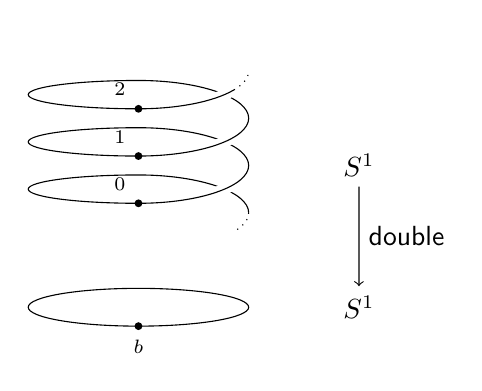
\begin{tikzpicture}[xscale=1.4,yscale=.6]
    \node (R) at (2,1) {$S^1$};
    \node (S1) at (2,-2) {$S^1$};
    \draw[->] (R) -- node[auto] {$\mathsf{double}$} (S1);
    \draw (0,-2) ellipse (1 and .4);
    \draw[dotted] (1,0) arc (0:-30:1 and .8);
    \draw (1,0) arc (0:90:1 and .8) arc (90:270:1 and .3) coordinate (t1);
    \draw[white,line width=4pt] (t1) arc (-90:90:1 and .8);
    \draw (t1) arc (-90:90:1 and .8) arc (90:270:1 and .3) coordinate (t2);
    \draw[white,line width=4pt] (t2) arc (-90:90:1 and .8);
    \draw (t2) arc (-90:90:1 and .8) arc (90:270:1 and .3) coordinate (t3);
    \draw[white,line width=4pt] (t3) arc (-90:90:1 and .8);
    \draw (t3) arc (-90:-30:1 and .8) coordinate (t4);
    \draw[dotted] (t4) arc (-30:0:1 and .8);
    \node[fill,circle,inner sep=1pt,label={below:\scriptsize $b$}] at (0,-2.4) {};
    \node[fill,circle,inner sep=1pt,label={above left:\scriptsize 0}] at (0,.2) {};
    \node[fill,circle,inner sep=1pt,label={above left:\scriptsize 1}] at (0,1.2) {};
    \node[fill,circle,inner sep=1pt,label={above left:\scriptsize 2}] at (0,2.2) {};
  \end{tikzpicture}
  \caption{The twisted double cover of $S^1$ in classical topology}\label{fig:winding}
\end{figure}
%
This important construction from homotopy theory is closely related to the celebrated Hopf fibration which, among other things, can be used to compute some of the higher homotopy groups of the spheres $S^2$ and $S^3$.  Indeed, one can construct the Hopf fibration in homotopy type theory in much the same way as the foregoing example, using univalence, negation, winding around the circle, and other constructions derived from combinations of logical, type-theoretic, and homotopical ideas.  

This sort of reasoning gives an entirely new ``synthetic" approach to some areas of classical mathematics like algebraic topology, which not only allows for the explicit logical formalization of classical results like the calculations of homotopy groups of spheres, but also permits their formal verification in computational proof systems based on a constructive system of logic.

\todo[inline]{OK, I'm happy with the the foregoing up to here (except for fixing the figure).  Now we need to do the
  conclusion using the notes that follow.  RH: agreed.}

An important point about univalent foundations is that it subsumes the classical set-theoretic framework for doing
mathematics.  The hierarchy of $n$-types neatly accounts for classical set-theoretic foundations within a broader
framework of homotopy types.  Specifically, $-1$-types, which have at most one element up to higher identification,
correspond to classical proof-irrelevant propositions, except that whether to insist that every proposition be inhabited
or empty remains a consistent choice that one may accept or reject at will.  The $0$-types, for which equality is a
classical proposition ($-1$-type) that is taken to be ``self-evident'' or ``proof-irrelevant'' correspond to classical
sets, without prior commitment to choice principles or whether membership is a boolean proposition; these can be taken
as axioms according to preference, without fear of inconsistency.  The advantage of univalent foundations is that
besides the familiar concepts of proposition (classically formalized as predicate calculus) and set (classically given
by the Zermelo-Fr\"{a}nkel axioms), it provides an infinite hierarchy of dimensions extending beyond just these two.
For example, the $1$-types are the natural setting for set-theoretic structures, such as groups or rings, that one may
wish to identify up to isomorphism.  Because two groups, say, can be isomorphic in different ways, the evidence for
their identification must provide the mutually inverse pairs of homomorpisms that constitute the identification.

Another import aspect of univalent foundations is that it extends Martin-L\"{o}f's type theory~\cite{mltt} with an
infinite hierarchy of dimensions that were hitherto inaccessible within the theory, even though models were known that
exhibited higher-dimensional structure~\cite{hofmann-streicher}.  Type theory was conceived as a foundation for
constructive mathematics, in which all constructions, including proofs of propositions, have direct computational
meaning in accordance with Brouwer's original program.  This connection with computation has proved enormously
influential in computer science, in particular in the theory of programming languages and the foundations of mechanized
proof.  At present homotopy type theory exploits the concept of proof relevance that is central to the constructivist
program (indeed, according to that program propositions are not just $-1$-types, but can be any $n$-type), and draws on
the emphasis on abstract types (for example, in the treatment of the identification type as an abstraction in itself,
rather than being encoded in terms of a concrete conception of homotopy).  The grand challenge is to extend the
computational interpretation to the full hierarchy of $n$-types, providing a computational meaning for, say, mappings
among higher-dimensional structures such as the spheres and toruses of arbitrary dimension.  Recent advances, such as
the development of a constructively valid model using cubical sets~\cite{bch}, strongly suggest that such a unification
is possible in the near future.  The implications for computer science are only beginning to be
explored~\cite{patch-theory}.

It is a curious fact, made all the more interesting by the above-mentioned developments, that two of the most successful
systems for mechanized proof, NuPRL~\cite{nuprl-book} and Coq~\cite{coq}, are based on constructive type theory.  Why
ought that be the case?  Univalent foundations seems to provide a clue, namely the importance of proof-relevance for
both classical homotopy theory and constructive mathematics.  A significant contribution of homotopy type theory is that
it exploits the axiomatic freedom of constructive mathematics (that is, the diminished emphasis on axioms that are
inconsistent, at full strength, with univalence) to achieve a synthetic formulation of homotopy theory that is wholly
coherent with constructive mathematics.  As Voevodsky has emphasized, classical theorem provers may only be used by
rather involved encodings of the natural concept of space using structures such as topological spaces or simplicial
sets, greatly impeding the process of formalization required to admit machine-checked proof.  This experiene parallels
the development of high-level (abstract) programming languages that provide a synthetic concept of computation, rather
than one based on low-level machine models such as the Turing machine or Random-Access Machine.  Thus we find that
whether we are discussing mechanized proof or verified programming, Church's $\lambda$-calculus emerges as a central
concept.  Perhaps this explains why constructive mathematics and mechanized proof are so tightly linked.


Some more things to mention:

- formal verification of mathematics as a practical tool makes logical foundations finally relevant to mathematical practice, rather than just a theoretical possibility.  In fact, if the latter is their only interest, then Goedel matters, but given the actual practical benefits, Goedel doesn't. This is a new "post-Goedel" attitude to logical foundations. 

- can something similar be said about foundations of computation ?  did people ever worry about Goedel the way the logicians do in connection with foundations of math?

- higher category theory turns out to be naturally described by constructive methods, while the subsystem of 0-categories (i.e. the sets) still admits classical logic, without forcing the higher dimensional part to also be classical.  This seems to be a new way of conceiving of the relation between classical and constructive methods -- not as distinct systems related to each other as "stronger versus weaker", or even as the different  logic of "constant versus variable" objects, but as compatible subsystems of a single system that are simultaneously applicable to different parts of the universe, distinguished by the intrinsic complexity or "dimension" of the objects therein.

we can close with saying that we are on the cusp of a revolution, in which two self-contained, well-motivated, well-justified, yet completely disparate frameworks for doing mathematics are not only being consolidated into a single, well-motivated, well-justified framework, but moreover the unified theory enriches and extends the classical framework without disrupting anything that has been achieved in that setting?

%%%%%%%%%%%%%%%%%%%%%%%%%%%%%%%%%%%%%%%%%%%%%%%%%%%%
\begin{thebibliography}{300}
%%%%%%%%%%%%%%%%%%%%%%%%%%%%%%%%%%%%%%%%%%%%%%%%%%%%

\bibitem{AW}
S.~Awodey and M.A.~Warren. Homotopy theoretic models of identity types. \emph{Math. Proc. Camb. Phil. Soc.}, 146, 45--55, 2009.

\bibitem{GvdB}
B.~van den Berg and R.~Garner. Topological and Simplicial Models of Identity Types. \emph{ACM Transactions on Computational Logic}, 13:1, 2012.

\bibitem{CwF} 
P.~Dybjer. ``Internal Type Theory." \emph{LNCS} 1158, 120--134, 1996.

\bibitem{HS} Hofman and Streicher 

\bibitem{HoTTbook} 
\emph{Homotopy Type Theory: Univalent Foundations of Mathematics}, The Univalent Foundations Program, Institute for Advanced Study, 2013. {\tt http://homotopytypetheory.org/book}

\bibitem{KLV}  
C.~Kapulkin, P.~LeFanu Lumsdaine and V.~Voevodsky, The Simplicial Model of Univalent Foundations. \emph{In preparation}, 2013.

%
\end{thebibliography}

%%%%%%%%%%%%%%%%%%%%%%%%%%%%%%%%%%%%%%%%%%%%%%%%%%%%
\end{document}
%%%%%%%%%%%%%%%%%%%%%%%%%%%%%%%%%%%%%%%%%%%%%%%%%%%%
